% ME4670J report starter. Compile with pdfLaTeX (Overleaf).
% Status: kinematic experiments verified; Webots validation pending.
% Replace this generic article layout with the official course template if supplied.
\documentclass[11pt,a4paper]{article}

\usepackage[margin=2.5cm]{geometry}
\usepackage[T1]{fontenc}
\usepackage[utf8]{inputenc}
\usepackage{lmodern}
\usepackage{amsmath,amssymb}
\usepackage{graphicx}
\usepackage{booktabs}
\usepackage{array}
\usepackage{microtype}
\usepackage{xcolor}
\usepackage{hyperref}
\usepackage{caption}
\usepackage{enumitem}
\hypersetup{colorlinks=true,linkcolor=blue!55!black,urlcolor=blue!55!black,citecolor=blue!55!black}
\graphicspath{{figures/}}
\newcommand{\pending}[1]{\textcolor{red!65!black}{\textbf{[TODO: #1]}}}
\newcommand{\methodname}{DWA-inspired velocity-sampling planner}

\title{Pedestrian-Aware Navigation for a Delivery Robot\\
\large ME4670J -- Robotics Project Report (Working Draft)}
\author{Anastasiia Ianke \and Sophia Olsson}
\date{\today}

\begin{document}
\maketitle
\noindent\textbf{Status note.} The experiments in this draft were run in a custom, idealized Python kinematic simulator. The Webots controller and world generator have been prepared but not executed in Webots. Do not label the results below as Webots results.

\begin{abstract}
This project examines whether short-horizon pedestrian motion prediction improves local navigation for a differential-drive delivery robot. We compare two otherwise identical velocity-sampling planners: a reactive planner that keeps pedestrian positions fixed throughout each candidate rollout, and a predictive planner using constant-velocity extrapolation from recent position measurements. In 120 reproducible trials from an idealized two-dimensional Python simulator, the predictive planner reached the goal in 45 of 60 cases, compared with 32 of 60 for the reactive planner. The respective collision counts were 15 and 28. Both planners frequently entered a predefined \(0.20\,\mathrm{m}\) pedestrian clearance margin. Among jointly successful trials, the median paired travel-time difference was \(0.0\,\mathrm{s}\) in each scenario family. These observations are limited to the kinematic simulator; Webots evaluation remains to be performed.
\end{abstract}

\section{Introduction and Research Question}
Delivery robots operating on shared walkways must move toward their destinations while responding to pedestrians. Reacting only to a pedestrian's present position can lead to late avoidance, whereas a motion forecast may fail when a pedestrian changes direction. We investigate the following question:
\begin{quote}
\emph{Under what conditions does short-horizon pedestrian motion prediction improve navigation efficiency without increasing collisions or unsafe proximity?}
\end{quote}
The project isolates local planning: the static walkway layout is known, pedestrians follow scripted motions, and positions are supplied directly by the simulator. Camera perception, mapping, learned models, and hardware tests are outside the present scope.

\section{Background and Relation to Course Concepts}
Our method is inspired by the Dynamic Window Approach (DWA) of Fox, Burgard, and Thrun~\cite{fox1997dwa}. It samples candidate velocity commands, evaluates short trajectories, and selects a command subject to geometric and kinematic constraints. It does \emph{not} reproduce all DWA safety admissibility conditions, and no formal collision-avoidance guarantee is claimed. Relevant course concepts include configuration space, coordinate frames, differential-drive forward kinematics, local planning, and feedback control. Webots and its Supervisor interface are the intended target simulator~\cite{webots_supervisor,webots_turtlebot}.

\section{System and Method}
\subsection{Robot model and collision representation}
The robot pose is \(\mathbf{q}=(x,y,\theta)\) with translational velocity \(v\) and yaw rate \(\omega\). The planar kinematics are
\begin{equation}
\dot{x}=v\cos\theta,\qquad \dot{y}=v\sin\theta,\qquad \dot{\theta}=\omega.
\label{eq:kinematics}
\end{equation}
With wheel radius \(r\) and wheel separation \(b\), commanded wheel angular velocities are
\begin{equation}
\dot{\phi}_L=\frac{v-b\omega/2}{r},\qquad
\dot{\phi}_R=\frac{v+b\omega/2}{r}.
\label{eq:wheels}
\end{equation}
For collision checking, the robot and each pedestrian are conservatively modeled as disks of radius \(0.20\,\mathrm{m}\) and \(0.18\,\mathrm{m}\), respectively. A pedestrian collision is recorded if their center distance becomes less than or equal to \(0.38\,\mathrm{m}\). Wall contacts are also recorded. Collision checking is discrete in time rather than continuous.

\subsection{Reactive and predictive pedestrian models}
Both planners use the same current positions, robot state, goal, candidate commands, objective function, and emergency deceleration rule. Only the future position model differs:
\begin{equation}
\hat{\mathbf{p}}_i(t+\tau)=
\begin{cases}
\mathbf{p}_i(t), & \text{reactive planner},\\
\mathbf{p}_i(t)+\hat{\mathbf{v}}_i(t)\tau, & \text{predictive planner}.
\end{cases}
\label{eq:pedprediction}
\end{equation}
The predictive velocity \(\hat{\mathbf{v}}_i\) is estimated from up to four recent observations using finite differences and capped at \(0.8\,\mathrm{m/s}\). Neither planner receives the pedestrian's future scripted path. The estimator associates observations by stable pedestrian ID, not by list ordering; new pedestrians initially have zero estimated velocity.

\subsection{Online velocity estimation (Sophia)}
For each pedestrian $i$, let $(t_a,\mathbf p_i(t_a))$ and $(t_b,\mathbf p_i(t_b))$ denote the oldest and newest samples in the rolling observation window. The velocity estimate is
\begin{equation}
\widetilde{\mathbf v}_i = \frac{\mathbf p_i(t_b)-\mathbf p_i(t_a)}{t_b-t_a}, \qquad
\hat{\mathbf v}_i=\widetilde{\mathbf v}_i
\min\left(1,\frac{v_{p,\max}}{\max(\lVert\widetilde{\mathbf v}_i\rVert,\varepsilon)}\right),
\end{equation}
where $v_{p,\max}=0.8\,\mathrm{m/s}$. Only samples from the present and past are used. Stable identifiers are required to avoid mixing tracks when people switch order in observations.

\subsection{Candidate trajectories and objective}
Every \(0.20\,\mathrm{s}\), a \methodname{} samples reachable forward and angular velocities and integrates candidate trajectories over a \(3.0\,\mathrm{s}\) horizon. We use \(v\leq0.18\,\mathrm{m/s}\), \(|\omega|\leq1.25\,\mathrm{rad/s}\), acceleration bounds of \(0.15\,\mathrm{m/s^2}\) and \(2.0\,\mathrm{rad/s^2}\), and wheel-speed limits of \(6.67\,\mathrm{rad/s}\). Candidates predicting contact are rejected. The remaining candidates are evaluated with
\begin{align}
J ={}& 8\,\Delta d_{\mathrm{goal}} + 0.28\cos(e_{\mathrm{heading}})
+2.8\,\mathrm{clip}(c_{\min},0,0.7)\notag\\
&+0.18v-0.04|\omega|-0.08|\Delta\omega|-0.03|\Delta v|,
\label{eq:score}
\end{align}
where \(\Delta d_{\mathrm{goal}}\) denotes goal-distance reduction and \(c_{\min}\) is minimum predicted boundary clearance. The scoring weights are heuristic. If no feasible candidate exists, the planner decelerates subject to the shared acceleration bound. This rule is not a safety guarantee.

\section{Implementation}
The common velocity sampler, collision checker, and robot geometry are implemented in \texttt{pednav/core.py}. Sophia's independent modules are in \texttt{pednav/sophia/}: \texttt{interface.py} (current-observation contract), \texttt{estimation.py} (ID-based velocity tracking), \texttt{controller.py} (planner adapter), and \texttt{analysis.py} (paired-run integrity checks and figures). Seeded pedestrian scenarios are in \texttt{pednav/scenarios.py}; the kinematic runner and metrics are in \texttt{pednav/runner.py}; and figure generation is in \texttt{pednav/analysis.py}. A local kinematic experiment driver produced the stored trial summary. The shared runner is in \texttt{pednav/runner.py}. Webots integration is a separate team workstream and has \emph{not} been verified as part of these reported experiments.

\section{Experimental Protocol}
We compare the planners in three scenario families: (i) a perpendicular crossing, (ii) an oncoming pedestrian with passing space, and (iii) a pedestrian that suddenly stops or turns. Each family uses seeds 5000--5019, paired across planners. This gives \(3\times20\times2=120\) kinematic runs. The stored kinematic dataset is intended as a preliminary comparison and must not substitute for independently verified Webots test trials. A \(3.0\,\mathrm{s}\) horizon replaced the \(2.0\,\mathrm{s}\) horizon proposed initially during development; Webots evaluation parameters still require joint agreement and freezing.

A run is a \emph{success} if the robot reaches within \(0.25\,\mathrm{m}\) of the goal without collision before a \(120\,\mathrm{s}\) timeout. We also log collisions, timeouts, path length, elapsed time, minimum pedestrian boundary clearance, time with commanded speed below \(0.01\,\mathrm{m/s}\), and whether clearance falls below the study's \(0.20\,\mathrm{m}\) monitoring threshold. This threshold is \emph{not} a certified safe distance. Time and path-length differences are assessed for paired cases where both planners succeed.

\section{Results: Verified Kinematic Simulation}
\begin{table}[htbp]
\centering
\caption{Results in the idealized Python kinematic simulator (20 cases per method and family). Counts refer to complete runs, not physical Webots trials.}
\label{tab:kinematic}
\small
\begin{tabular}{@{}lrrrrrr@{}}
\toprule
& \multicolumn{2}{c}{Successes} & \multicolumn{2}{c}{Collisions} & \multicolumn{2}{c}{Clearance $<0.20$ m}\\
\cmidrule(lr){2-3}\cmidrule(lr){4-5}\cmidrule(l){6-7}
Scenario & R & P & R & P & R & P\\
\midrule
Crossing & 6 & 9 & 14 & 11 & 17 & 17\\
Oncoming & 20 & 20 & 0 & 0 & 20 & 18\\
Stop/turn & 6 & 16 & 14 & 4 & 20 & 18\\
\midrule
Total & 32 & 45 & 28 & 15 & 57 & 53\\
\bottomrule
\end{tabular}
\end{table}

Across all three families, the reactive planner succeeded in \(32/60\) trials and the predictive planner in \(45/60\). There were \(28/60\) and \(15/60\) collisions, respectively, and no timeouts. Clearance fell below \(0.20\,\mathrm{m}\) in \(57/60\) reactive and \(53/60\) predictive runs. These measured outcomes support a narrower claim of fewer recorded disk-overlap collisions in this test harness, not real-world safety.

\begin{figure}[htbp]
\centering
\IfFileExists{figures/outcomes.png}{%
  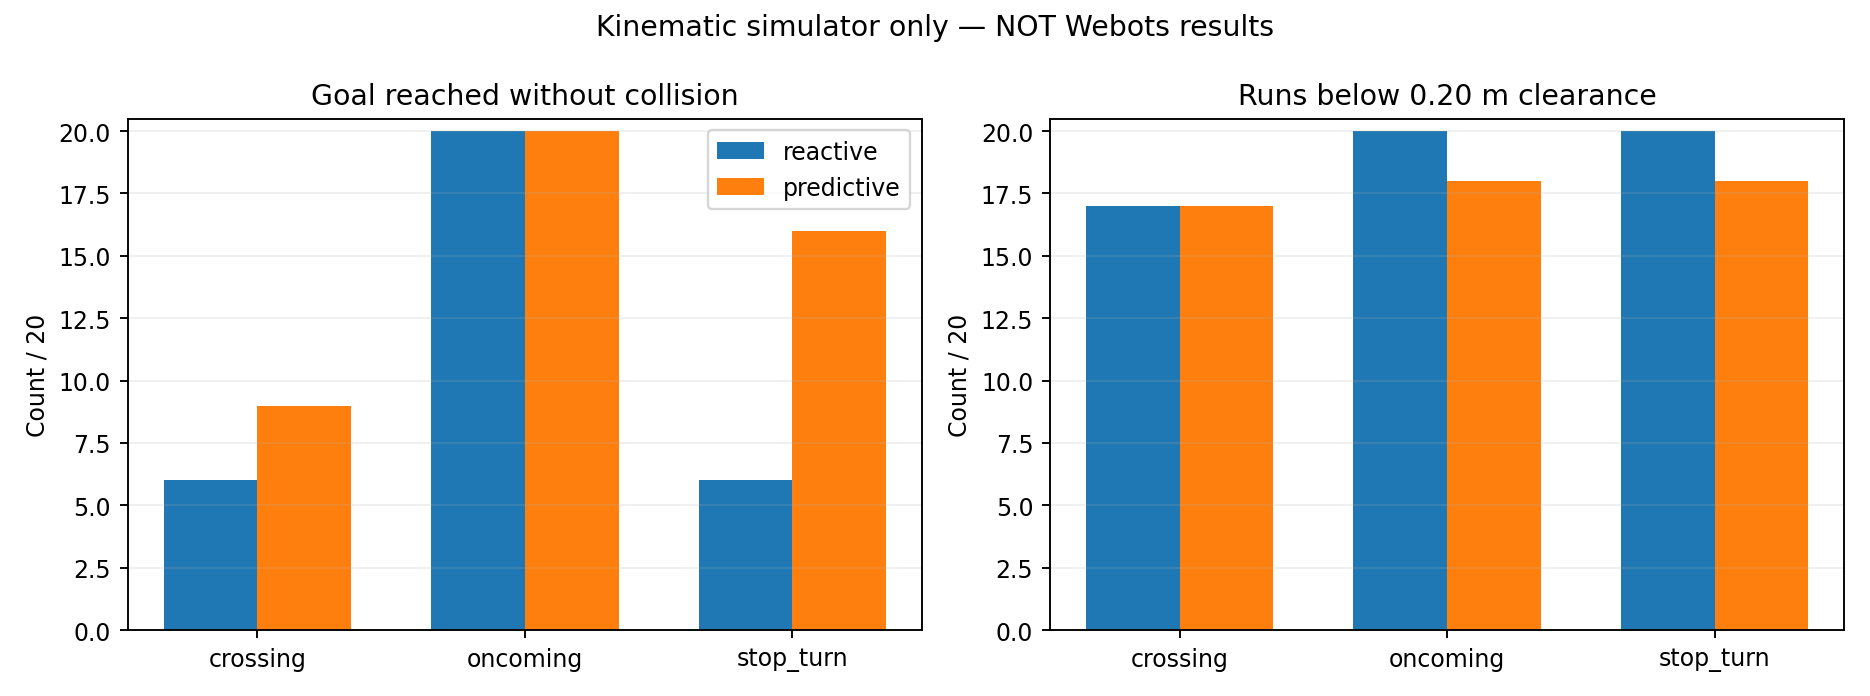
\includegraphics[width=0.95\linewidth]{outcomes.png}%
}{\fbox{\parbox{0.85\linewidth}{Figure pending: upload \texttt{figures/outcomes.png}}}}
\caption{Observed success and close-proximity outcomes in the Python kinematic test harness. Not Webots data.}
\label{fig:outcomes}
\end{figure}

Both planners succeeded in six paired crossing trials, 20 oncoming trials, and three stop/turn trials. Among jointly successful pairs, the median predictive-minus-reactive travel-time difference was \(0.0\,\mathrm{s}\) in each family. Median path-length differences were approximately \(-0.0009\,\mathrm{m}\) (crossing), \(+0.0057\,\mathrm{m}\) (oncoming), and \(0\,\mathrm{m}\) (stop/turn). Consequently, the current kinematic evidence does not establish faster goal completion for the predictive model when both methods succeed.

\begin{figure}[htbp]
\centering
\IfFileExists{figures/paired_times.png}{%
  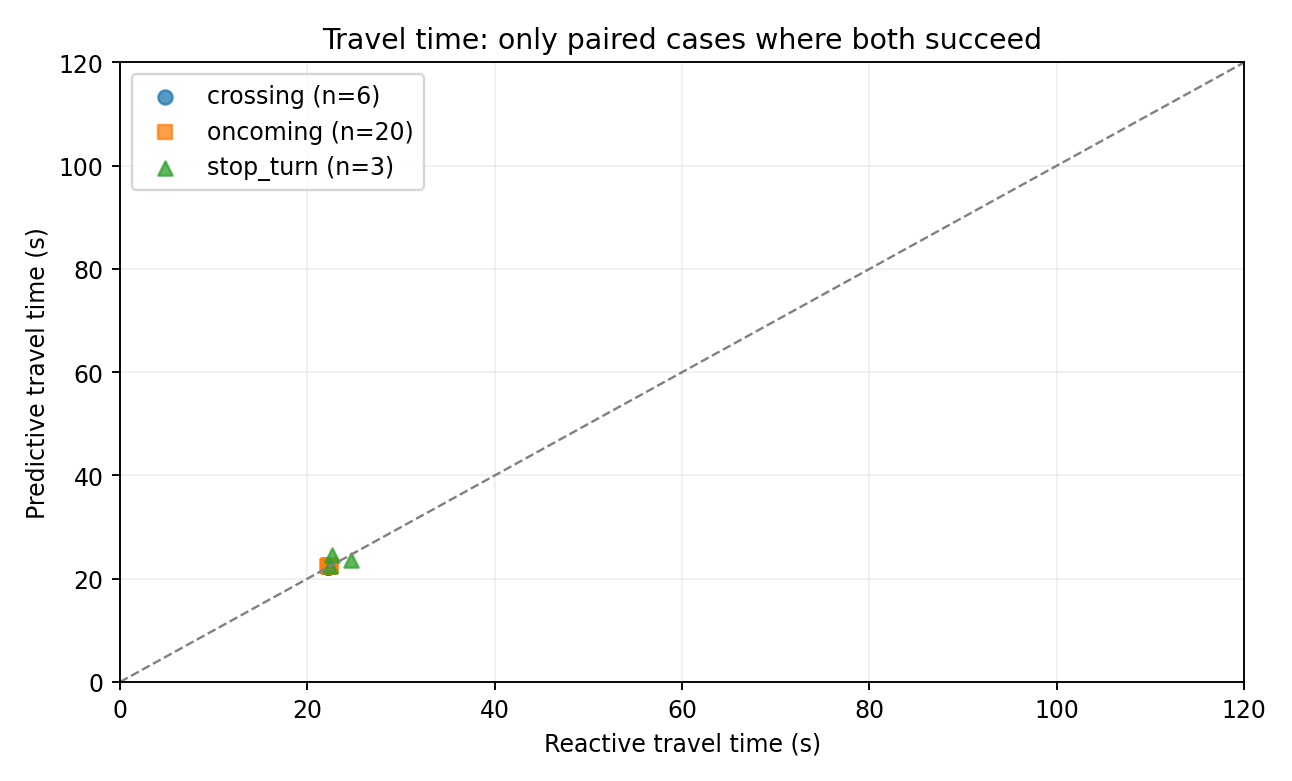
\includegraphics[width=0.95\linewidth]{paired_times.png}%
}{\fbox{\parbox{0.85\linewidth}{Figure pending: upload \texttt{figures/paired\_times.png}}}}
\caption{Travel-time comparisons restricted to paired cases where both methods succeeded in the kinematic simulation.}
\label{fig:times}
\end{figure}

\section{Discussion and Limitations}
The main observed benefit of prediction in the idealized experiments is a greater number of successful goal arrivals and fewer collisions, notably in stop/turn cases. This was not accompanied by a median travel-time reduction among jointly successful pairs. Close encounters were common for both planners, which is important evidence against making broad safety claims. The scripted pedestrian motions and idealized robot kinematics omit perception noise, latency, physical contacts, and human responses. Position errors and a \(3.0\,\mathrm{s}\) linear extrapolation may be especially problematic when pedestrians abruptly change motion. Because collision checks occur only at \(0.20\,\mathrm{s}\) intervals, contacts between samples can be missed.

\section{Webots Validation: Pending}
\pending{Execute at least one matched reactive/predictive Webots pair; verify wheel directions and robot movement.}

\pending{After compatibility checks, run the defined Webots scenario set and report actual success, collision, timeout, clearance and timing values separately from Table~\ref{tab:kinematic}.}

\pending{Add authentic Webots screenshots or video frames, cite run seeds, and discuss any differences from idealized kinematics.}

\section{Conclusion}
The implemented Python framework provides a reproducible comparison between a reactive and a constant-velocity-predictive local planner. Across 120 idealized kinematic runs, prediction was associated with more goal arrivals and fewer recorded geometric collisions, but not a median paired travel-time gain; frequent clearance-threshold violations also remain. These results cannot yet be generalized to Webots dynamics or real-world robot safety. The next milestone is a measured Webots evaluation.

\section*{Author Contributions and AI Assistance}
\pending{Replace this proposed split with the students' actual, verified contributions.} The original proposal lists Anastasiia Ianke and Sophia Olsson as project members. Proposed tasks were scenario generation, reactive baseline and logging for Anastasiia, and velocity prediction, integration and analysis for Sophia, with joint review and presentation. Software scaffolding, analysis scripts and draft text have been produced with AI assistance; students must review, reproduce and disclose such assistance as required by the course.

\begin{thebibliography}{9}
\bibitem{fox1997dwa}
D. Fox, W. Burgard, and S. Thrun, ``The Dynamic Window Approach to Collision Avoidance,'' \emph{IEEE Robotics \& Automation Magazine}, vol. 4, no. 1, pp. 23--33, 1997. DOI: \href{https://doi.org/10.1109/100.580977}{10.1109/100.580977}.

\bibitem{webots_supervisor}
Cyberbotics, ``Webots Supervisor API Reference.'' \url{https://github.com/cyberbotics/webots/blob/master/docs/reference/supervisor.md}.

\bibitem{webots_turtlebot}
Cyberbotics, ``TurtleBot3Burger.proto,'' Webots R2025a source. \url{https://github.com/cyberbotics/webots/blob/R2025a/projects/robots/robotis/turtlebot/protos/TurtleBot3Burger.proto}.
\end{thebibliography}
\end{document}
